\documentclass{pretexto/report}
% --- Archivo de bibliografía -----------------
\addbibresource{pretexto/repbib.bib}

\def\fillandplacepagenumber{%
 \par\pagestyle{empty}%
 \vbox to 0pt{\vss}\vfill
 \vbox to 0pt{\baselineskip0pt
   \hbox to\linewidth{\hss}%
   \baselineskip\footskip
   \hbox to\linewidth{%
     \hfil\thepage\hfil}\vss}}


\title{Análisis y diseño}

%%%%%%%%%%%%%%%%%%%% TERMINA PREÁMBULO %%%%%%%%%%%%

\begin{document}

%%%%%%%%%%%%%%%%%%%% PORTADA %%%%%%%%%%%%%%%%%%%%%%%

\begin{titlepage}
  \thispagestyle{empty}
  \pagecolor{white}
  
  % Encabezado con logos
  \begin{center}
    \vspace{1cm}
    
    % Logos en la parte superior
   
      \centering
          \vspace{2cm}
      
\includegraphics[height=2.35cm]{img/logos.png}
    
    \vspace{3cm}
    
    % Tipo de trabajo
    {\normalsize\color{charcoal}\textsc{Tarea}}\\[0.5cm]
    
    % Título principal
    {\huge\bfseries\color{black}Análisis y Diseño de software}\\[0.5cm]

    
    \vspace{1.5cm}
    
    % Información de autores
    {\small\color{charcoal}\textsc{Realizada por}}\\[0.3cm]
    
    {\normalsize\color{black}Robles Guzmán Naomi Isabel}\\[0.2cm]
    {\normalsize\color{black}Ugalde Téllez Aarón}\\[0.5cm]

    
    \vspace{0.8cm}
    
    % Información académica
    {\small\color{charcoal}\textsc{Para la materia de}}\\[0.2cm]
    {\normalsize\color{blue}Ingeniería de Software para Sistemas Inteligentes}\\[0.5cm]
    
    {\small\color{charcoal}\textsc{Impartida por}}\\[0.2cm]
    {\normalsize\color{black}Chadwick Carreto Arellano}\\[0.5cm]
    
    {\small \color{charcoal}\textsc{Grupo}}\\[0.3cm]
    {\normalsize\color{black}6BM1}\\[0.8cm]
    
    \vfill
    
    % Línea decorativa y fecha
    {\color{blue}\rule{0.4\textwidth}{1pt}}\\[0.3cm]
    {\large\color{charcoal}03 de octubre de 2025}
    
    \vspace{1cm}
    
  \end{center}
\end{titlepage}                                                     

%%%%%%%%%%%%%%%%%%%% ÍNDICES %%%%%%%%%%%%%%%%%%%%%%%%%%
\tableofcontents 
\pagebreak


%%%%%%%%%%%%%%%%% INTRODUCCIÓN %%%%%%%%%%%%%%%%%%%%%%%%

\pagebreak


\section{Objetivos}

\begin{itemize}
    \item Desarrollar un sistema que permita al usuario registrar sus habitos y tareas diarias
    \item Añadir espacios para que el usuario agregue datos que sirvan de contexto para las recomendaciones inteligentes.
    \item Implementar un modulo que realice recomendaciones inteligentes sobre como realizar los habitos y tareas registradas
    \item Realizar una interfaz intuitiva y atractiva que permita añadir las tareas y habitos de manera facil
\end{itemize}


\section{Diagrama Entidad-Relación}
\begin{figure}[H]
    \centering
    \includegraphics[width=\linewidth]{pngs/relacional.png}
    \caption{Diagrama generado de Entidad Relación}
\end{figure}

\section{Diagrama de Procesos}
\begin{figure}[H]
    \centering
    \includegraphics[height=\textwidth]{pngs/procesos.png}
    \caption{Diagrama de procesos}
\end{figure}

\subsection{Descripción del Diagrama de Flujo de Proceso}
El diagrama representa el flujo completo de procesos del sistema de gestión de tareas académicas, 
organizado en una estructura jerárquica que abarca desde el acceso inicial hasta la generación de 
recomendaciones personalizadas.

\subsubsection{Proceso de Acceso y Registro}
El flujo inicia con el acceso del usuario al sistema mediante una decisión condicional que determina 
si el usuario está registrado. En caso negativo, el sistema direcciona al proceso de registro donde 
se capturan datos empresariales (nombre, email, contraseña y grado académico). Posteriormente, 
se procede con la validación de datos y la creación de cuenta, seguida del envío de un email de 
verificación.
\subsubsection{Proceso de Autenticación}
Para usuarios registrados, el sistema solicita credenciales de login (email y contraseña) y valida 
su autenticidad. Una vez autenticado exitosamente, se verifica si existen credenciales correctas, 
tras lo cual se crea el dashboard principal del sistema.

\subsubsection{Gestión de Tareas}
El dashboard principal proporciona tres rutas principales de acción:
\begin{itemize}
\item \textbf{Gestión de Perfil:} Permite actualizar información personal mediante la captura de datos como nombre,
 foto de perfil y país.
\item \textbf{Visualización por Categoría:} Organiza las tareas en categorías predefinidas y muestra las mismas 
por fecha.
\item \textbf{Proceso de Creación de Tareas:} Incluye la captura de información (título, descripción, fecha límite
 y categoría), seguida de una decisión sobre el uso de servicios de terceros para obtener videos de YouTube o
  artículos de referencia.
\end{itemize}

\subsubsection{Proceso de Recomendaciones}
El sistema implementa un módulo de recomendaciones inteligente que permite al usuario decidir si requiere feedback.
 Este módulo integra:
\begin{itemize}
\item Ingreso de datos de tarea (título, descripción, URL de recurso académico, tipo de contenido y fuente)
\item Ingresar casos de tareas exitosas, recomendaciones previas y observaciones
\item Proceso de creación de tareas relacionadas con las recomendaciones
\item Almacenamiento de recomendaciones guardadas
\item Generación de recomendaciones finales con opción de registrar feedback
\end{itemize}
\subsubsection{Flujos de Salida}
El sistema cuenta con múltiples puntos de salida que conducen al cierre de sesión (90 días de inactividad) 
o finalización de procesos específicos, manteniendo la coherencia del flujo mediante conectores visuales 
que unifican las diferentes rutas del proceso.

\section{Diagramas de Casos de Uso}
\subsection{Autenticación y perfil}
\begin{figure}[H]
    \centering
    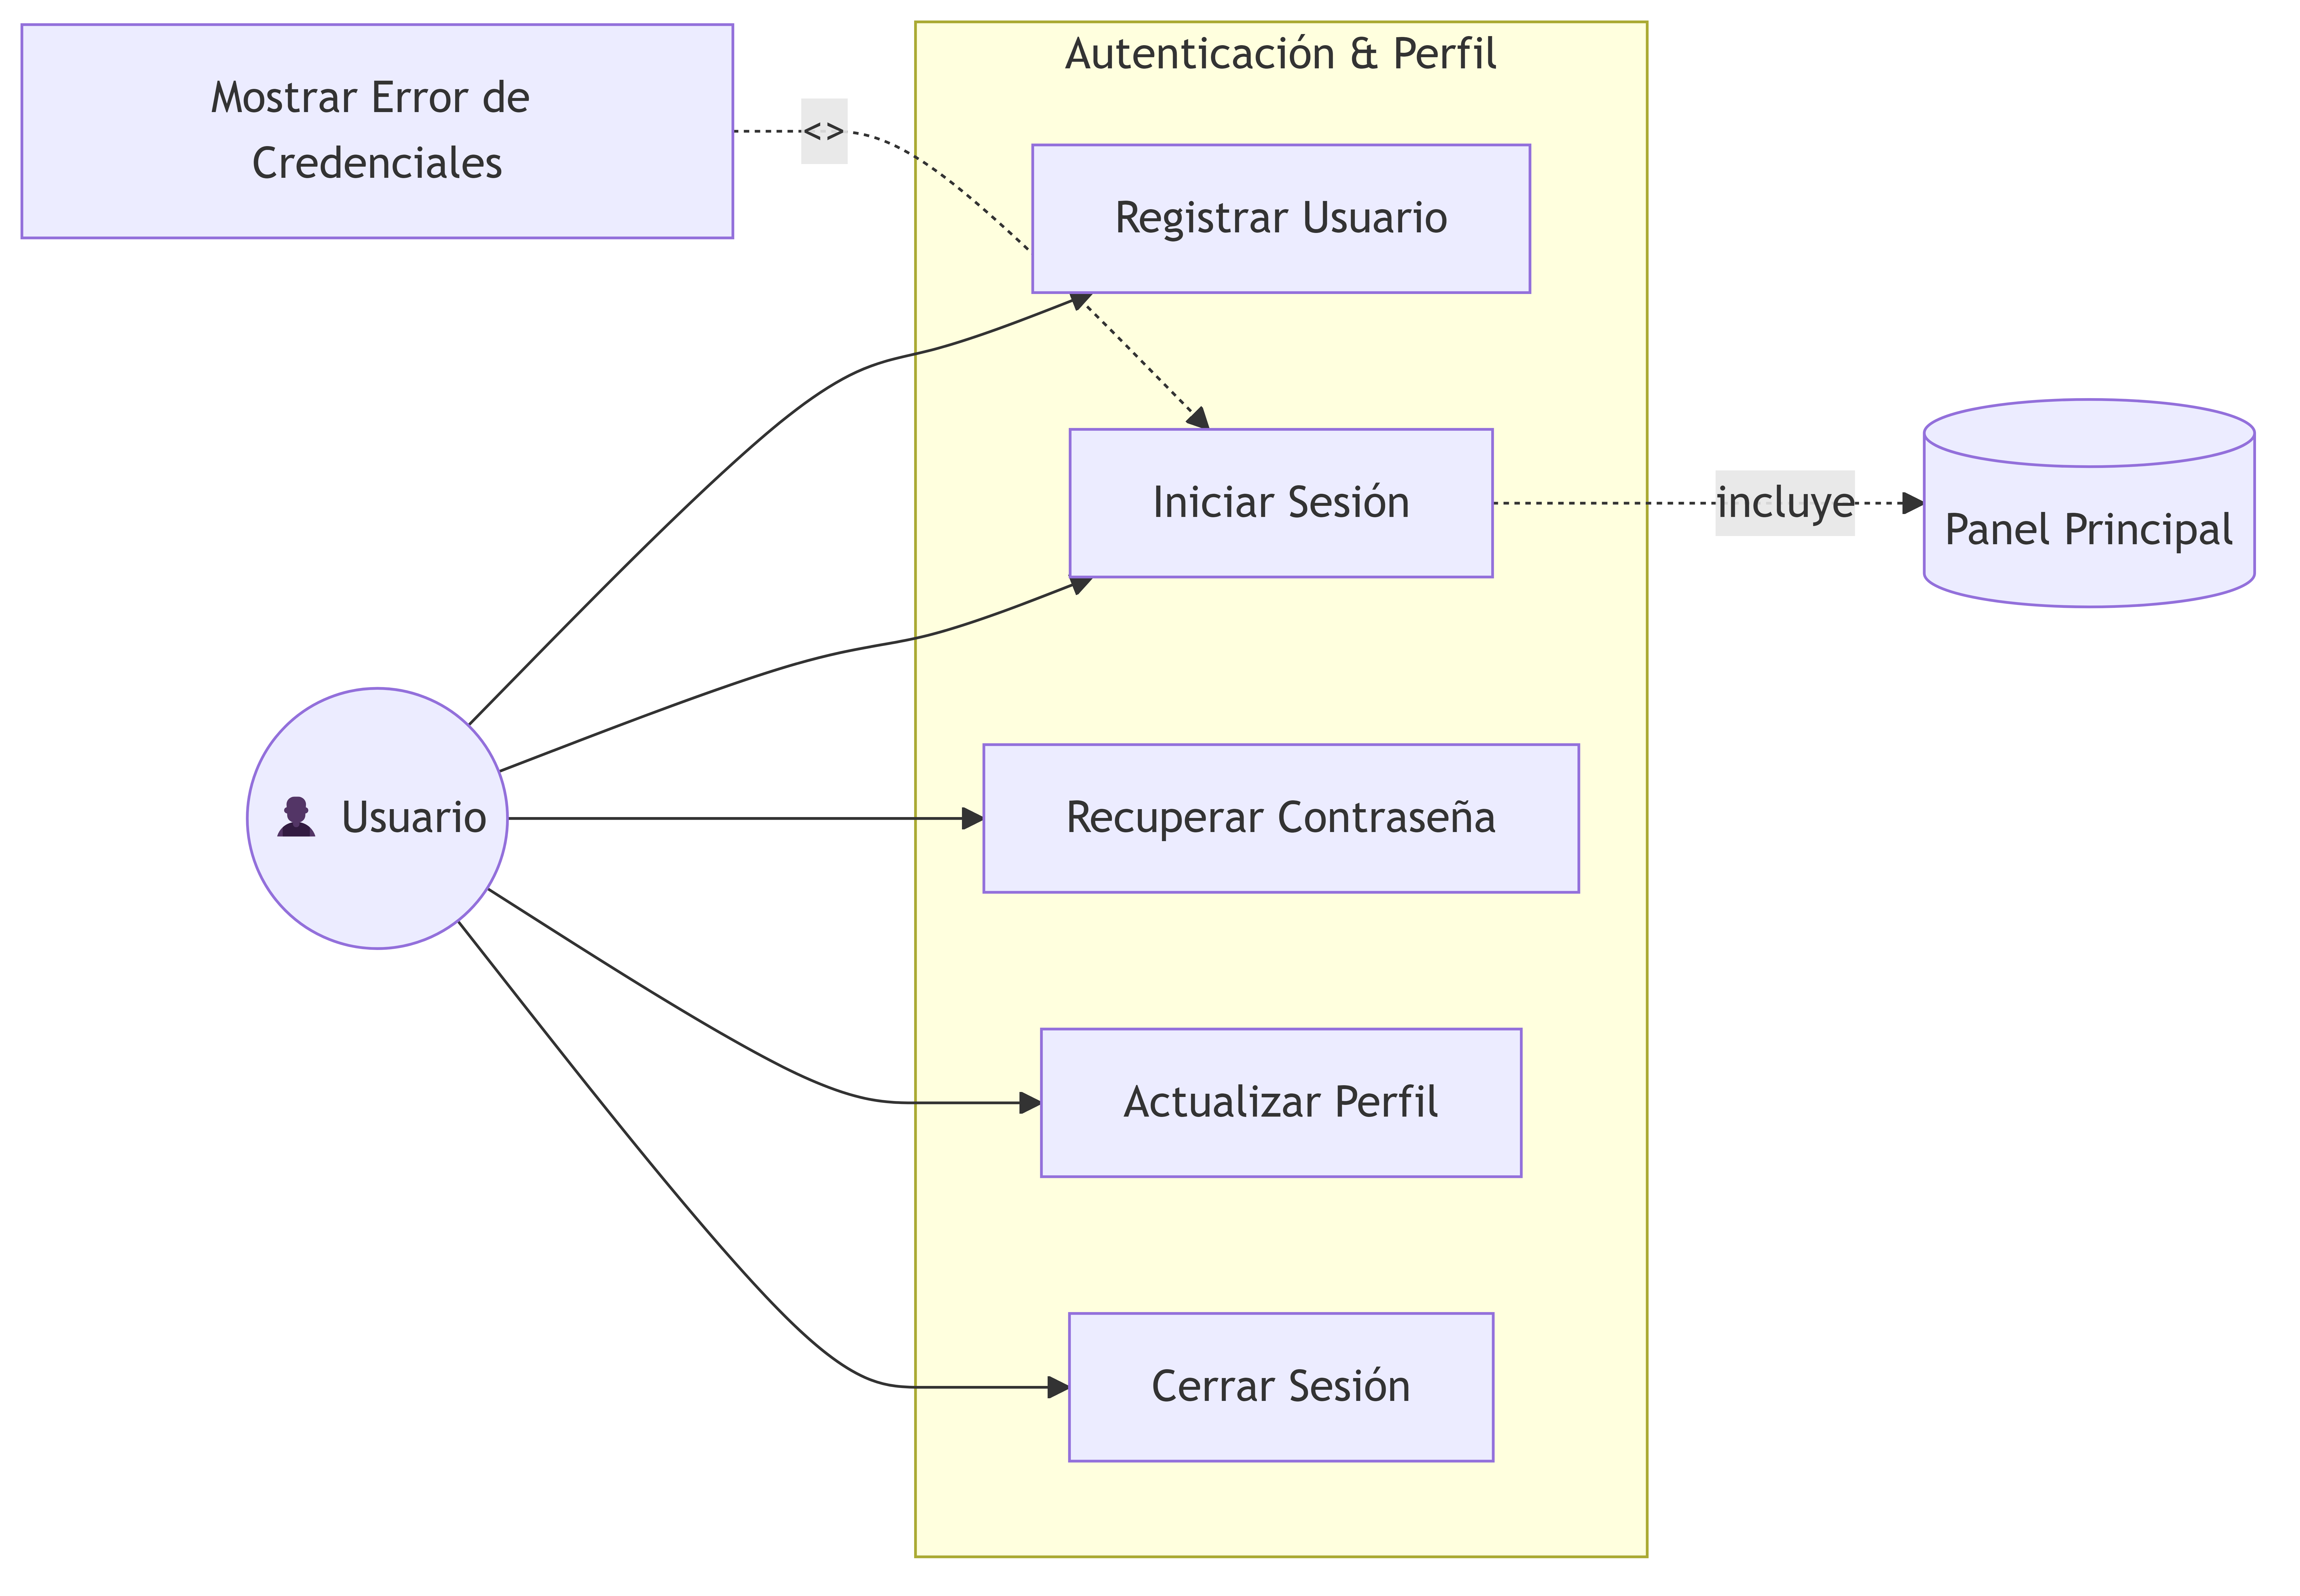
\includegraphics[width=0.7\linewidth]{pngs/uc_1.png}
    \caption{Caso de uso 1: Autenticación y Perfil}
\end{figure}

\subsection{Gestión de Tareas}
\begin{figure}[H]
    \centering
    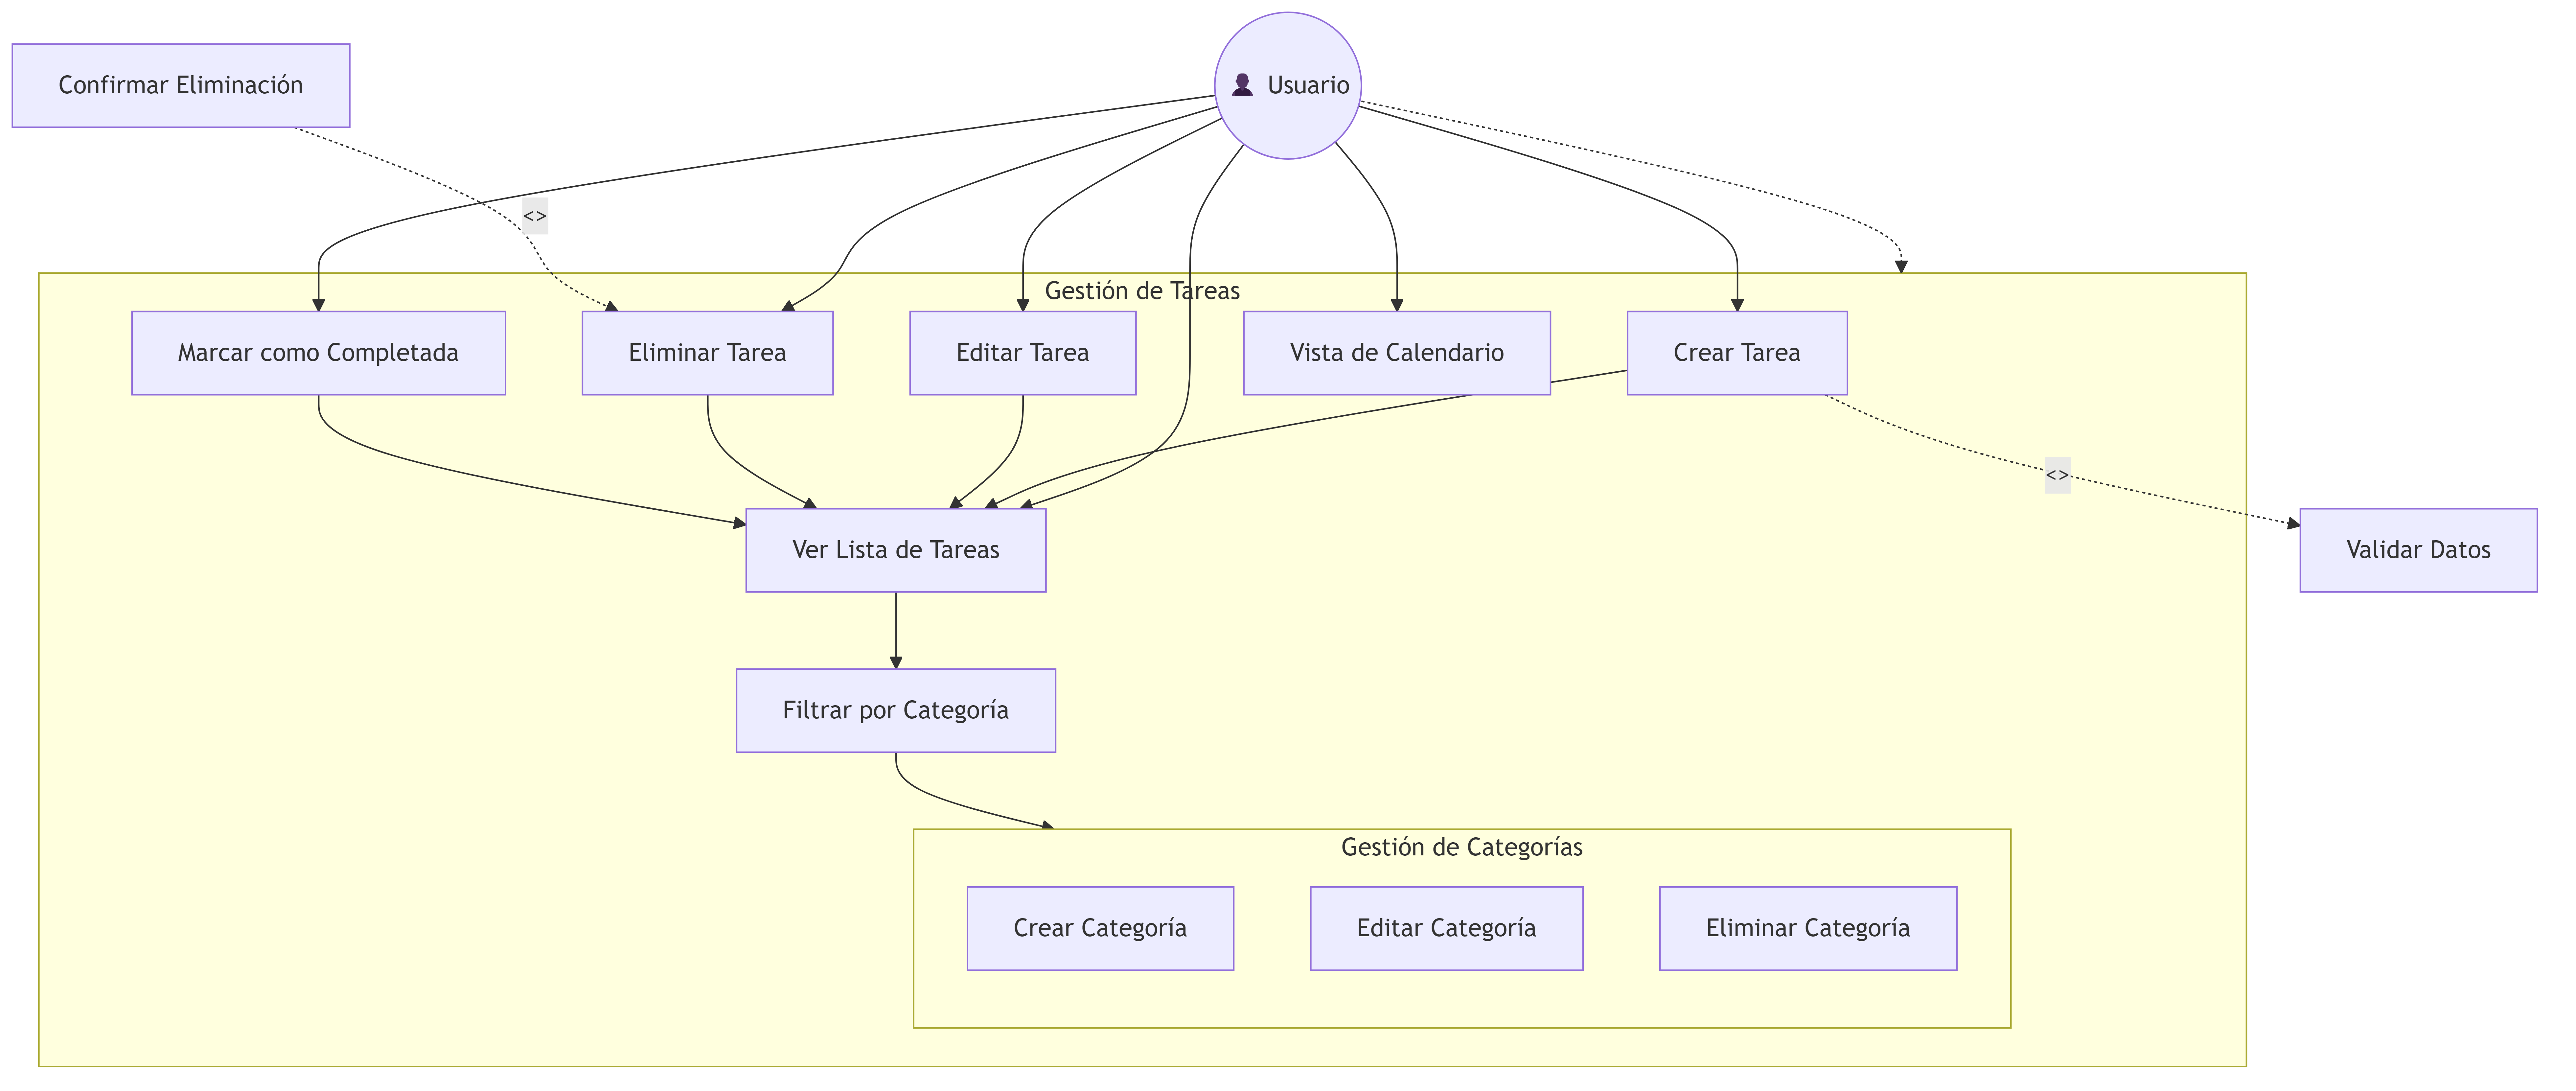
\includegraphics[width=0.9\linewidth]{pngs/uc_2.png}
    \caption{Caso de uso 2: Gestión de Tareas}
\end{figure}
\subsection{Recomendaciones}
\begin{figure}[H]
    \centering
    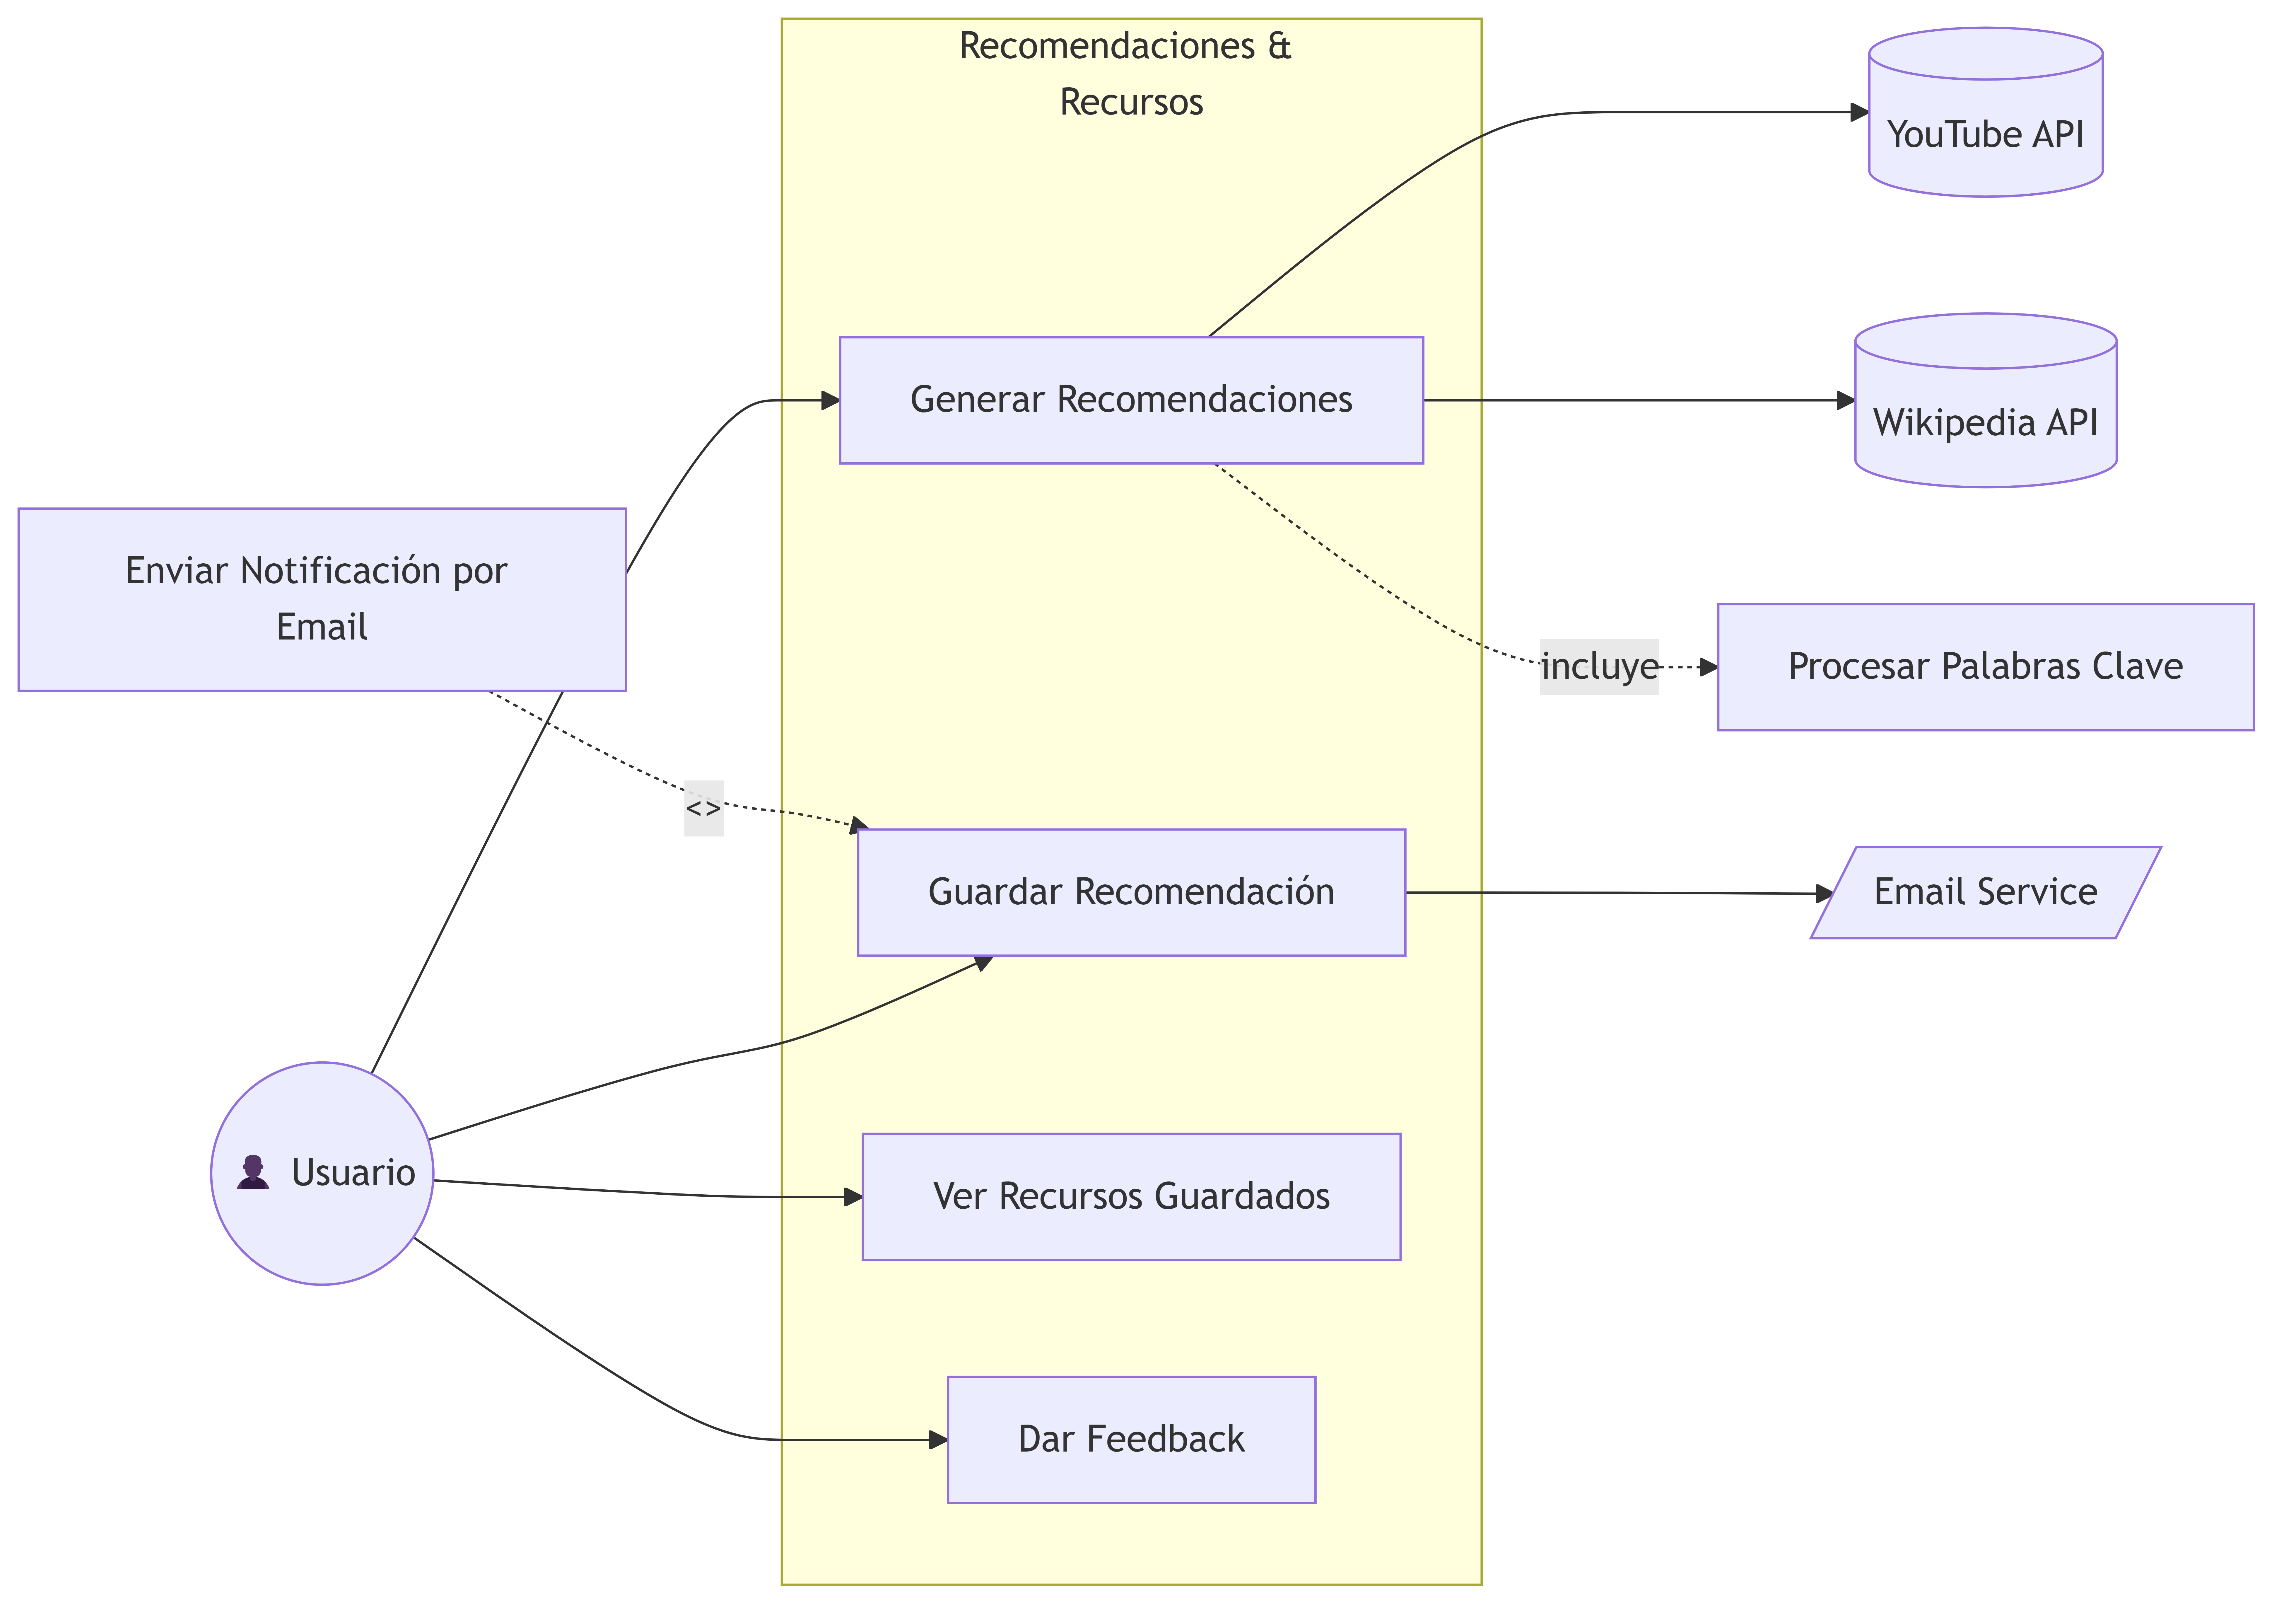
\includegraphics[width=0.7\linewidth]{pngs/uc_3.png}
    \caption{Caso de uso 3: Recomendaciones y Recursos (APIs externas)}
\end{figure}
\subsection{Administración}
\begin{figure}[H]
    \centering
    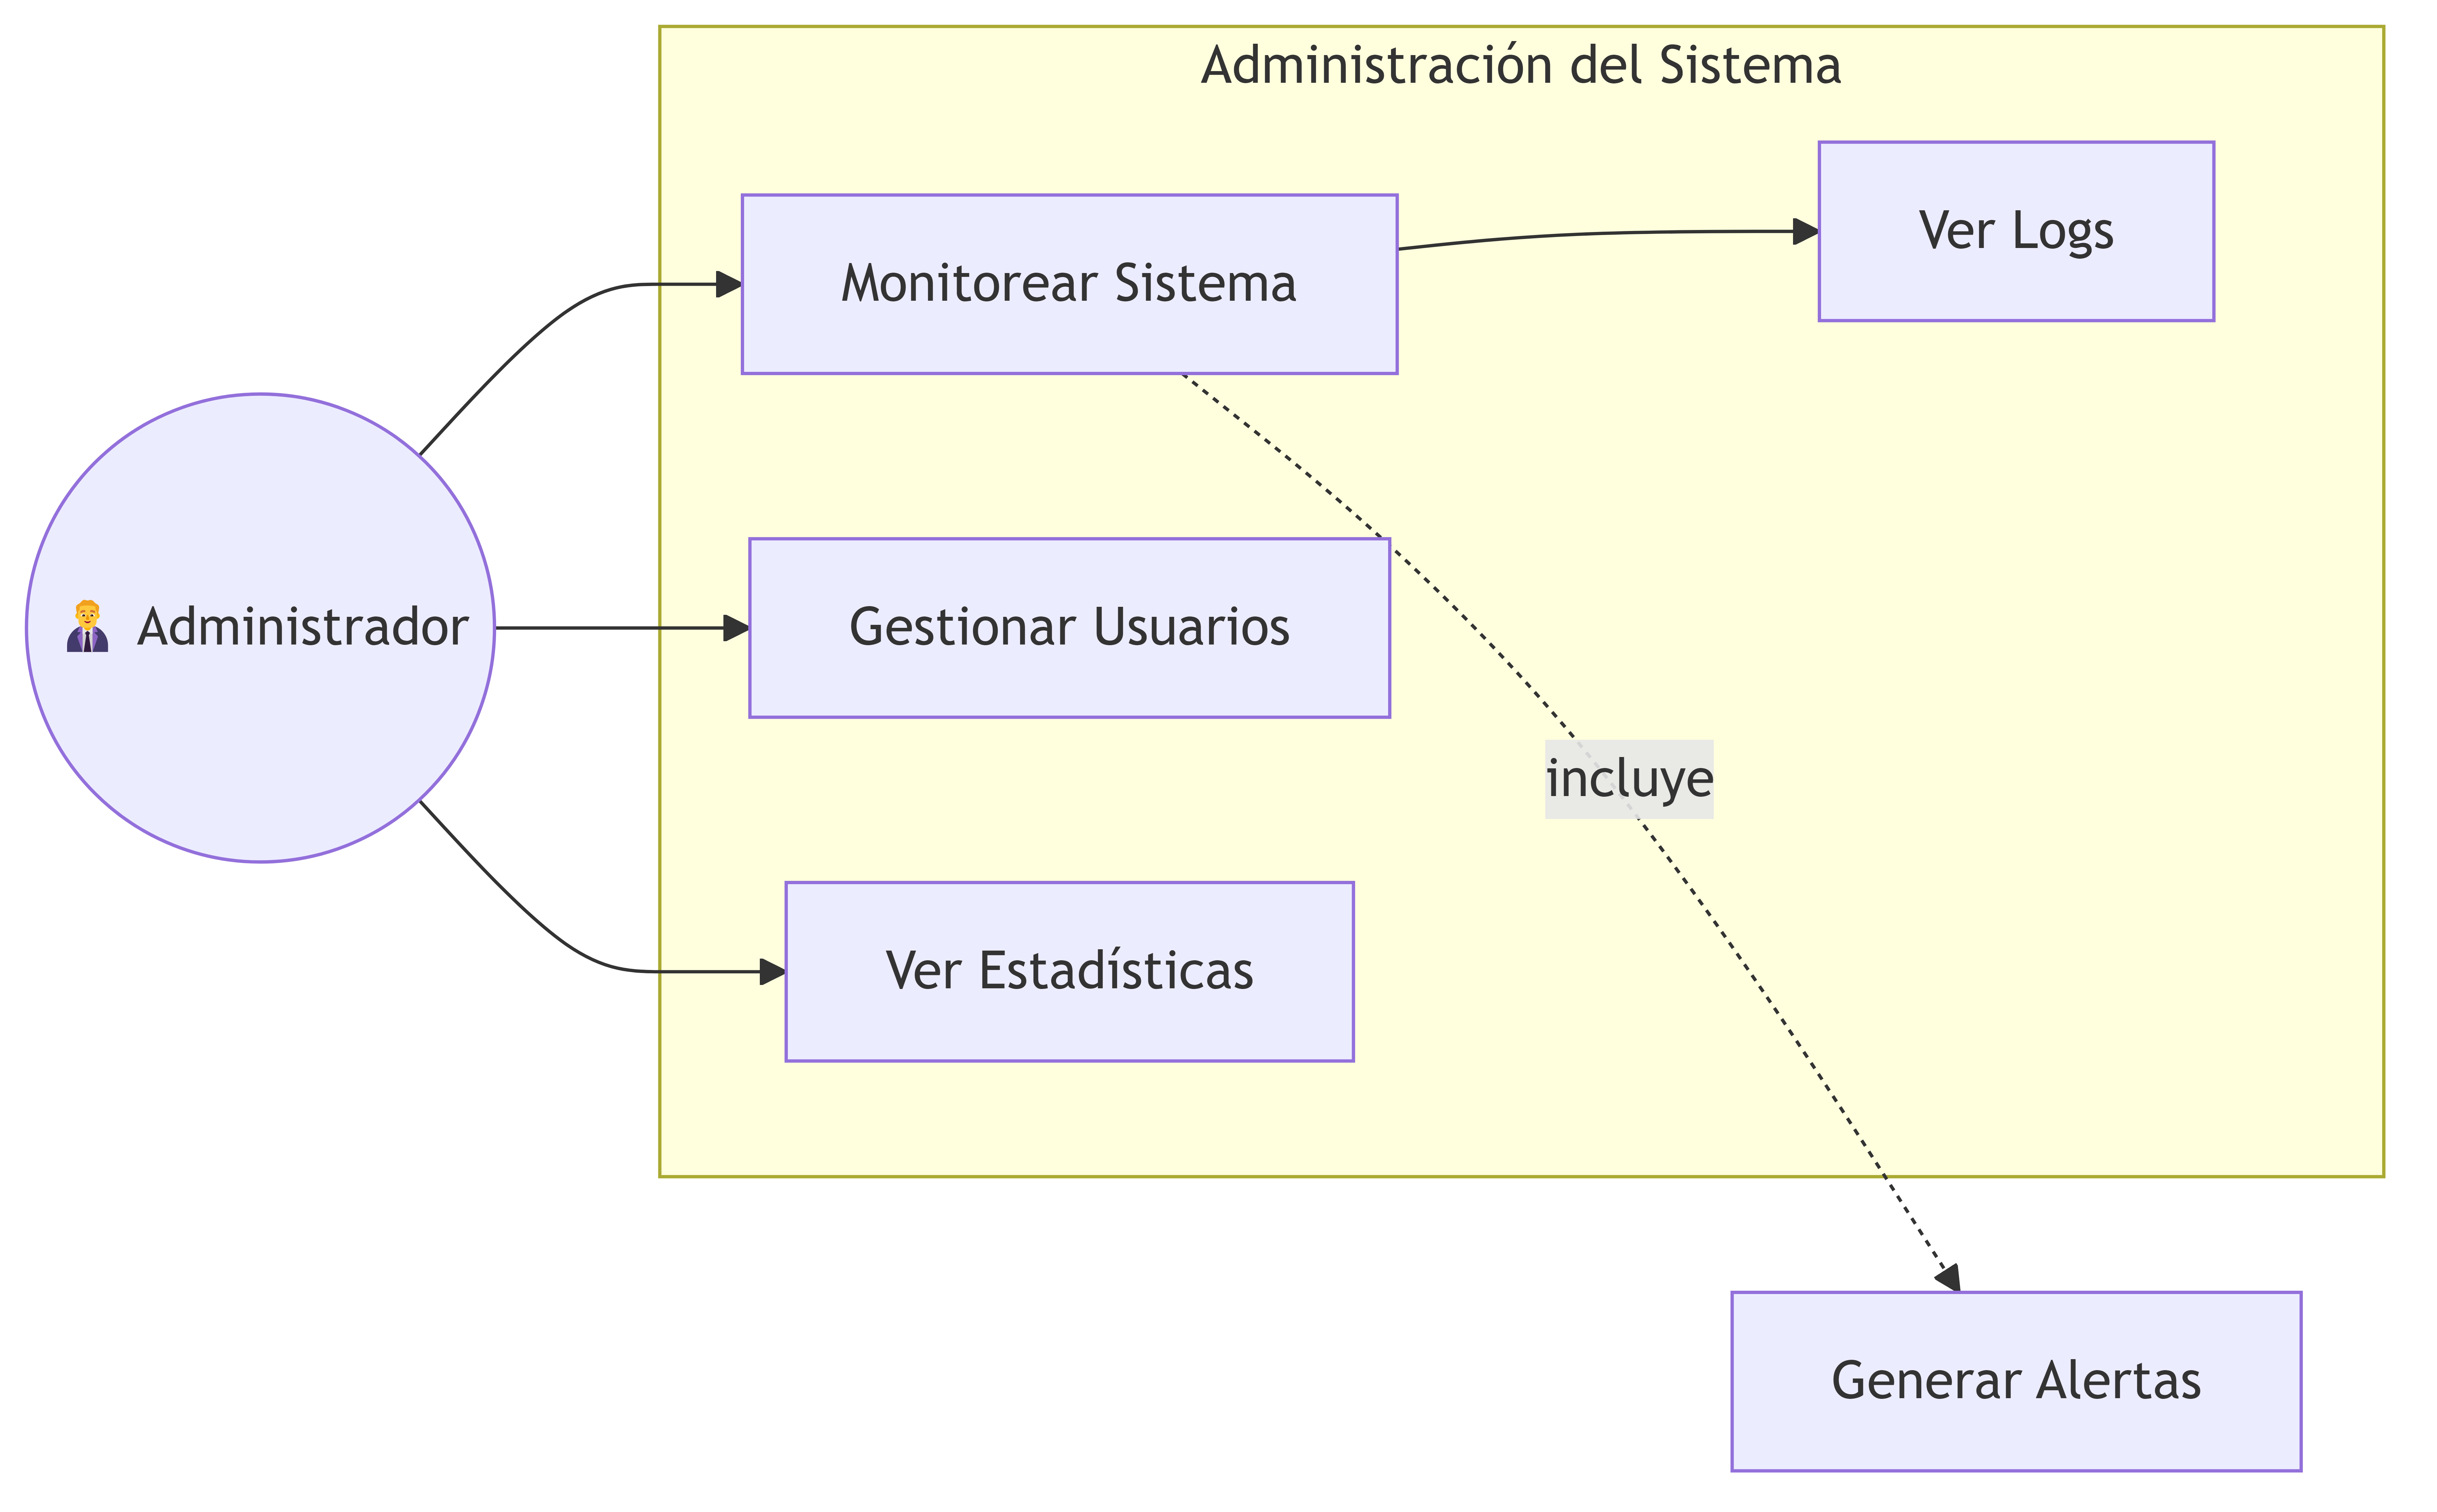
\includegraphics[width=0.7\linewidth]{pngs/uc_4.png}
    \caption{Caso de uso 4: Administración}
\end{figure}

\begin{landscape}
\landscapefancy

\section{Diagrama de Entradas y Salidas}
\begin{figure}[H]
    \centering
    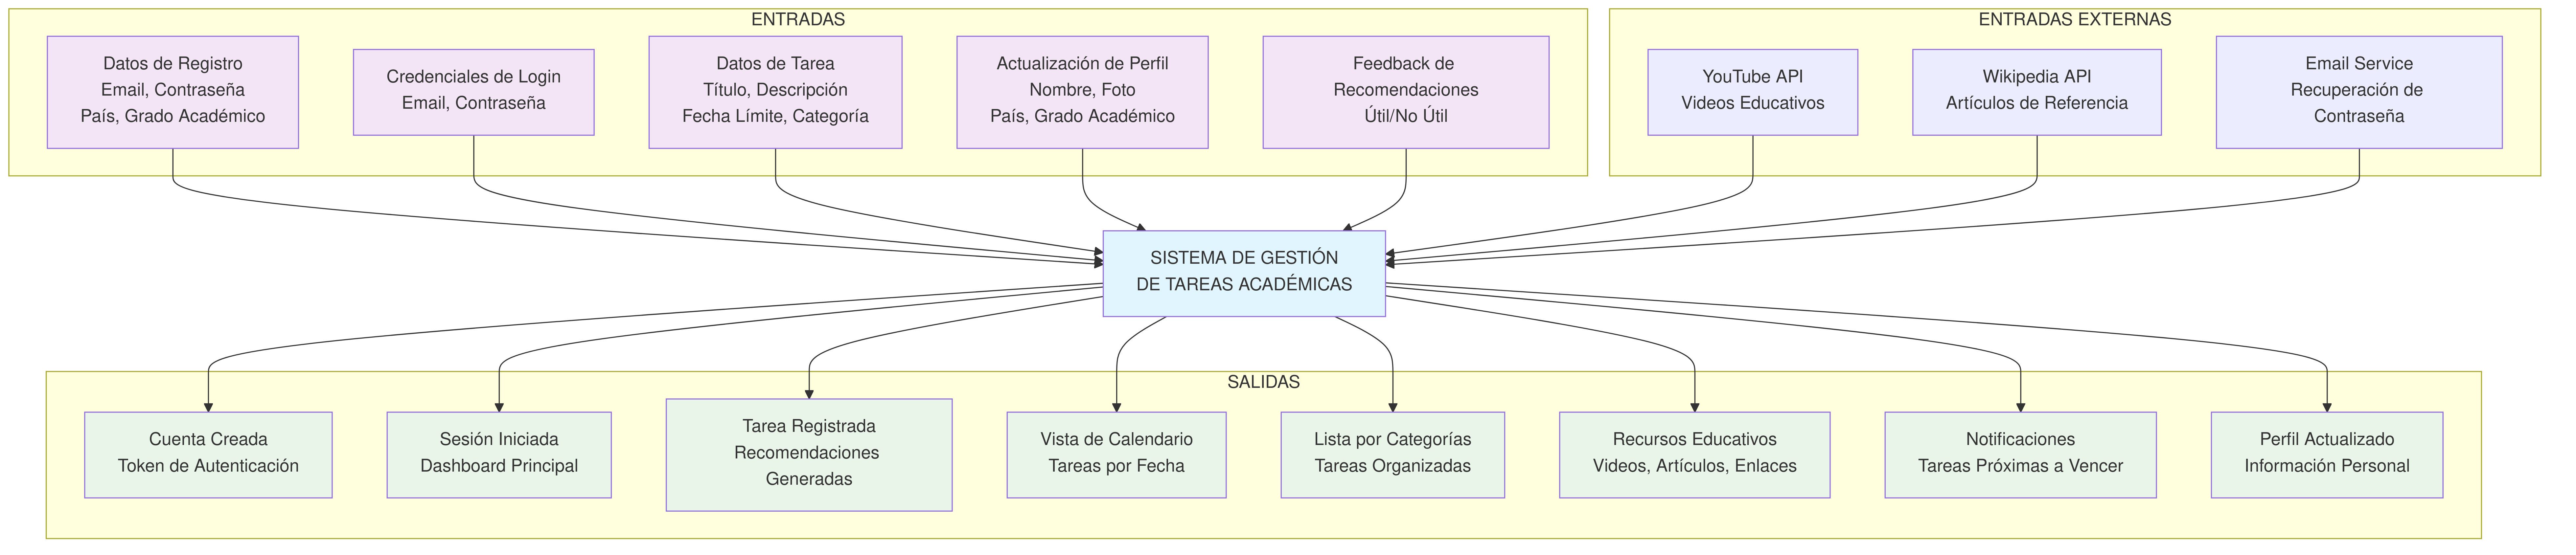
\includegraphics[width=\linewidth]{pngs/e_s.png}
    \caption{Diagrama de entradas y salidas}
\end{figure}

\section{Diagrama de Arquitectura de Software}
\begin{figure}[H]
    \centering
    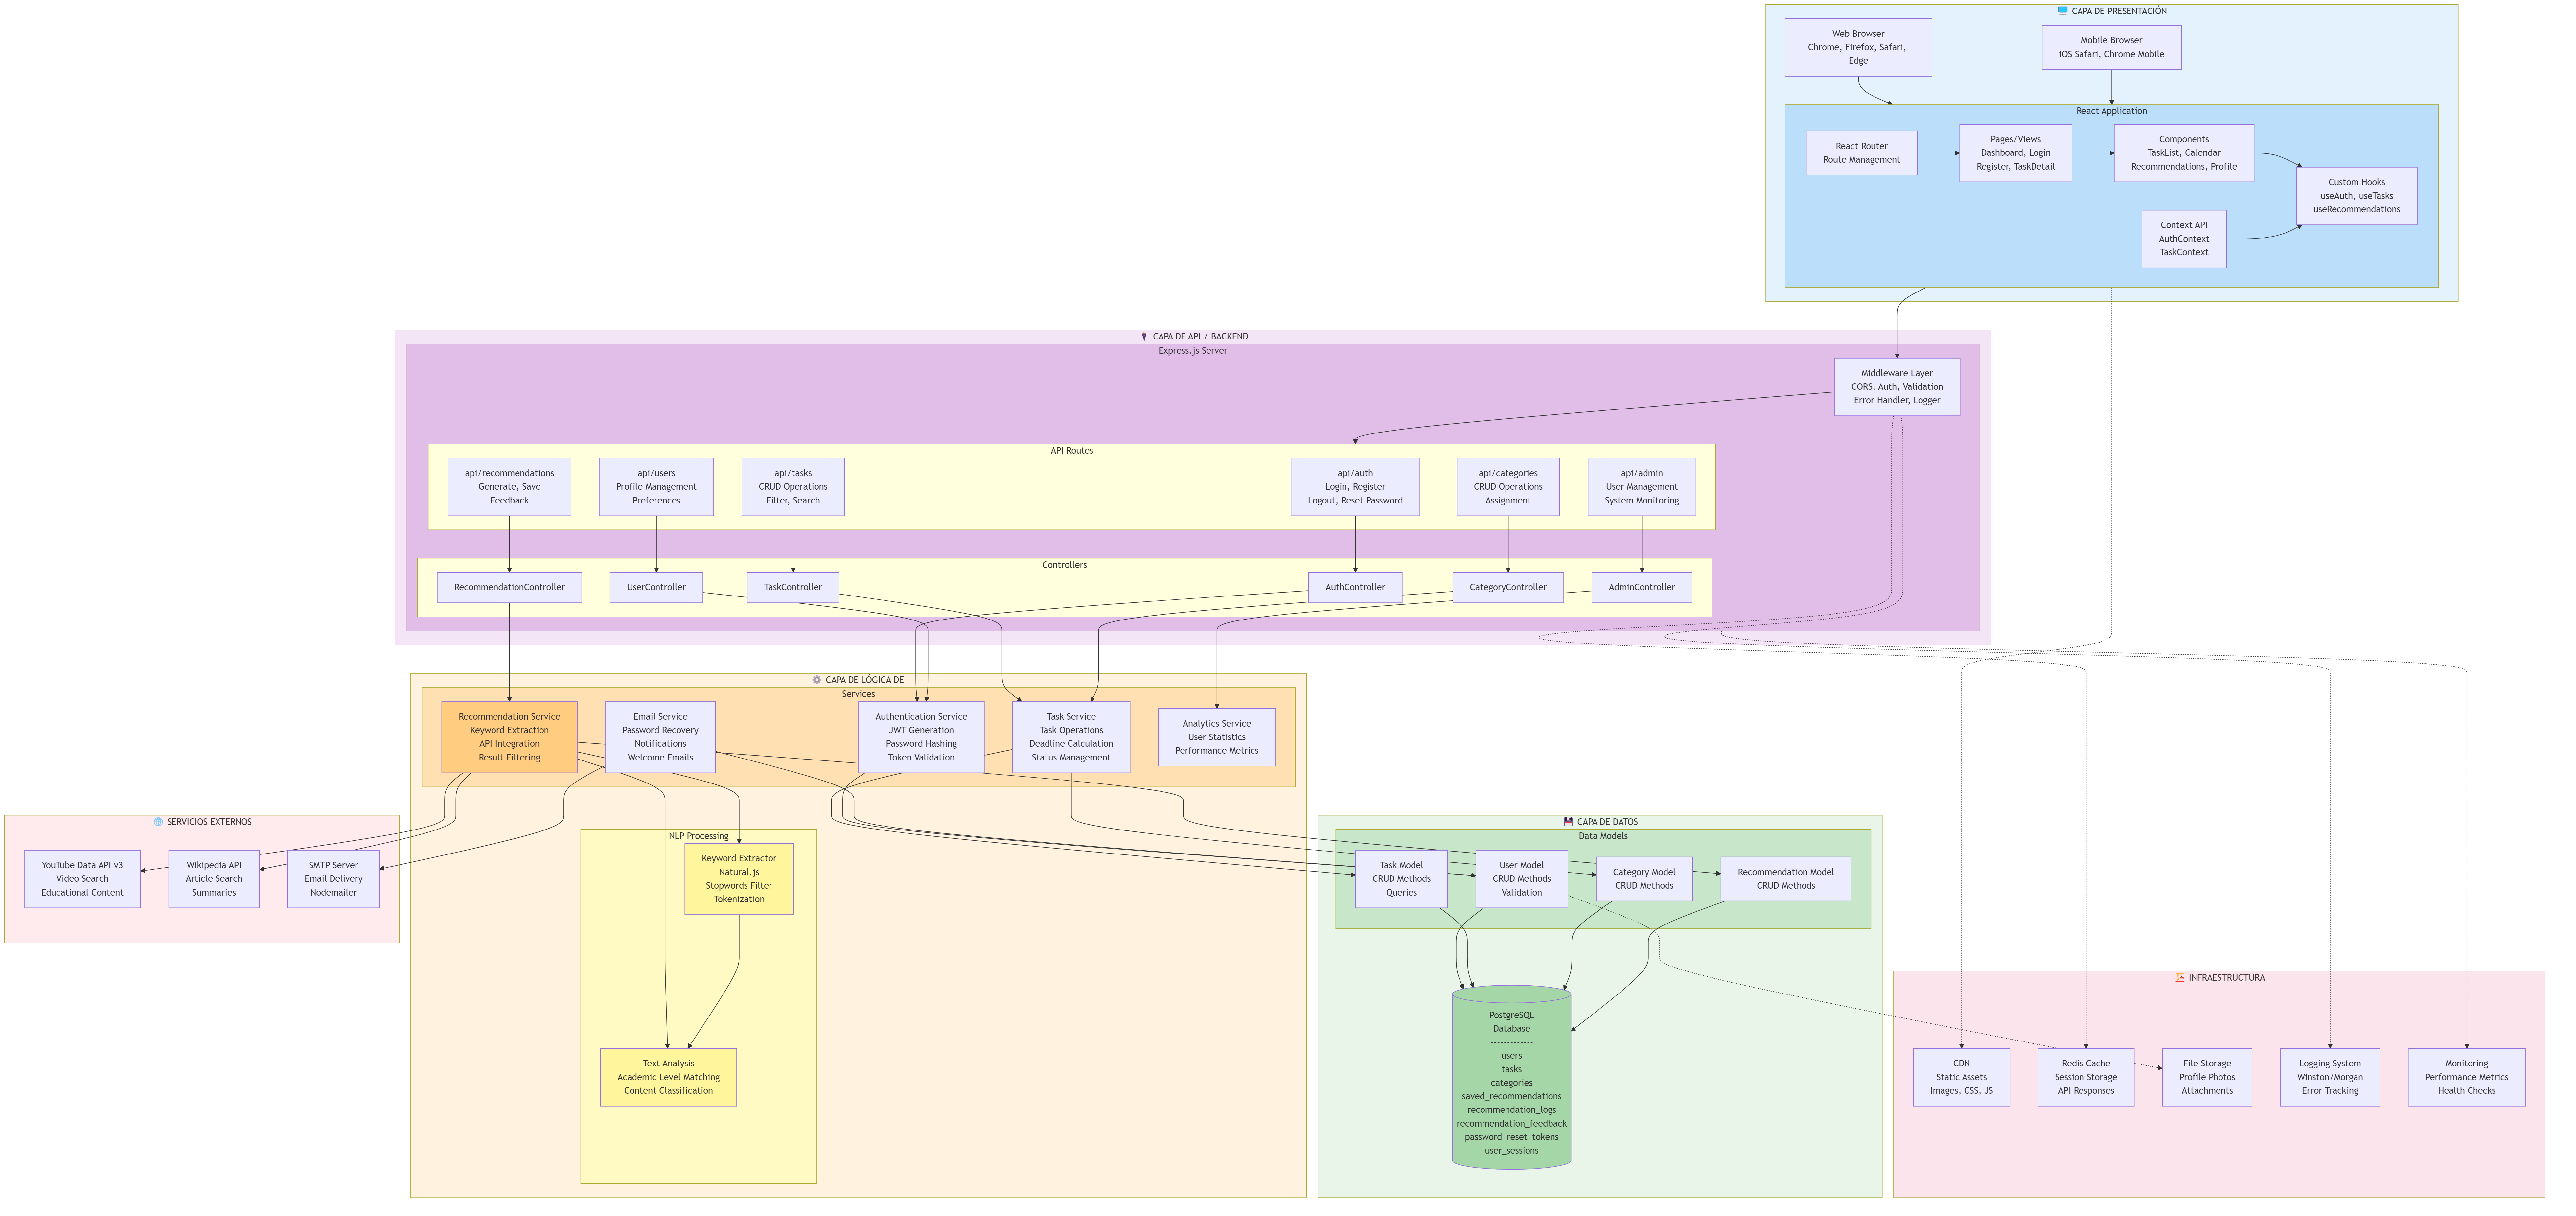
\includegraphics[width=\linewidth]{pngs/arquitectura.png}
    \caption{Diagrama de arquitectura de software}
\end{figure}

\end{landscape}

\section{Maqueta de la Interfaz de Usuario}
\begin{figure}[H]
    \centering
    \fbox{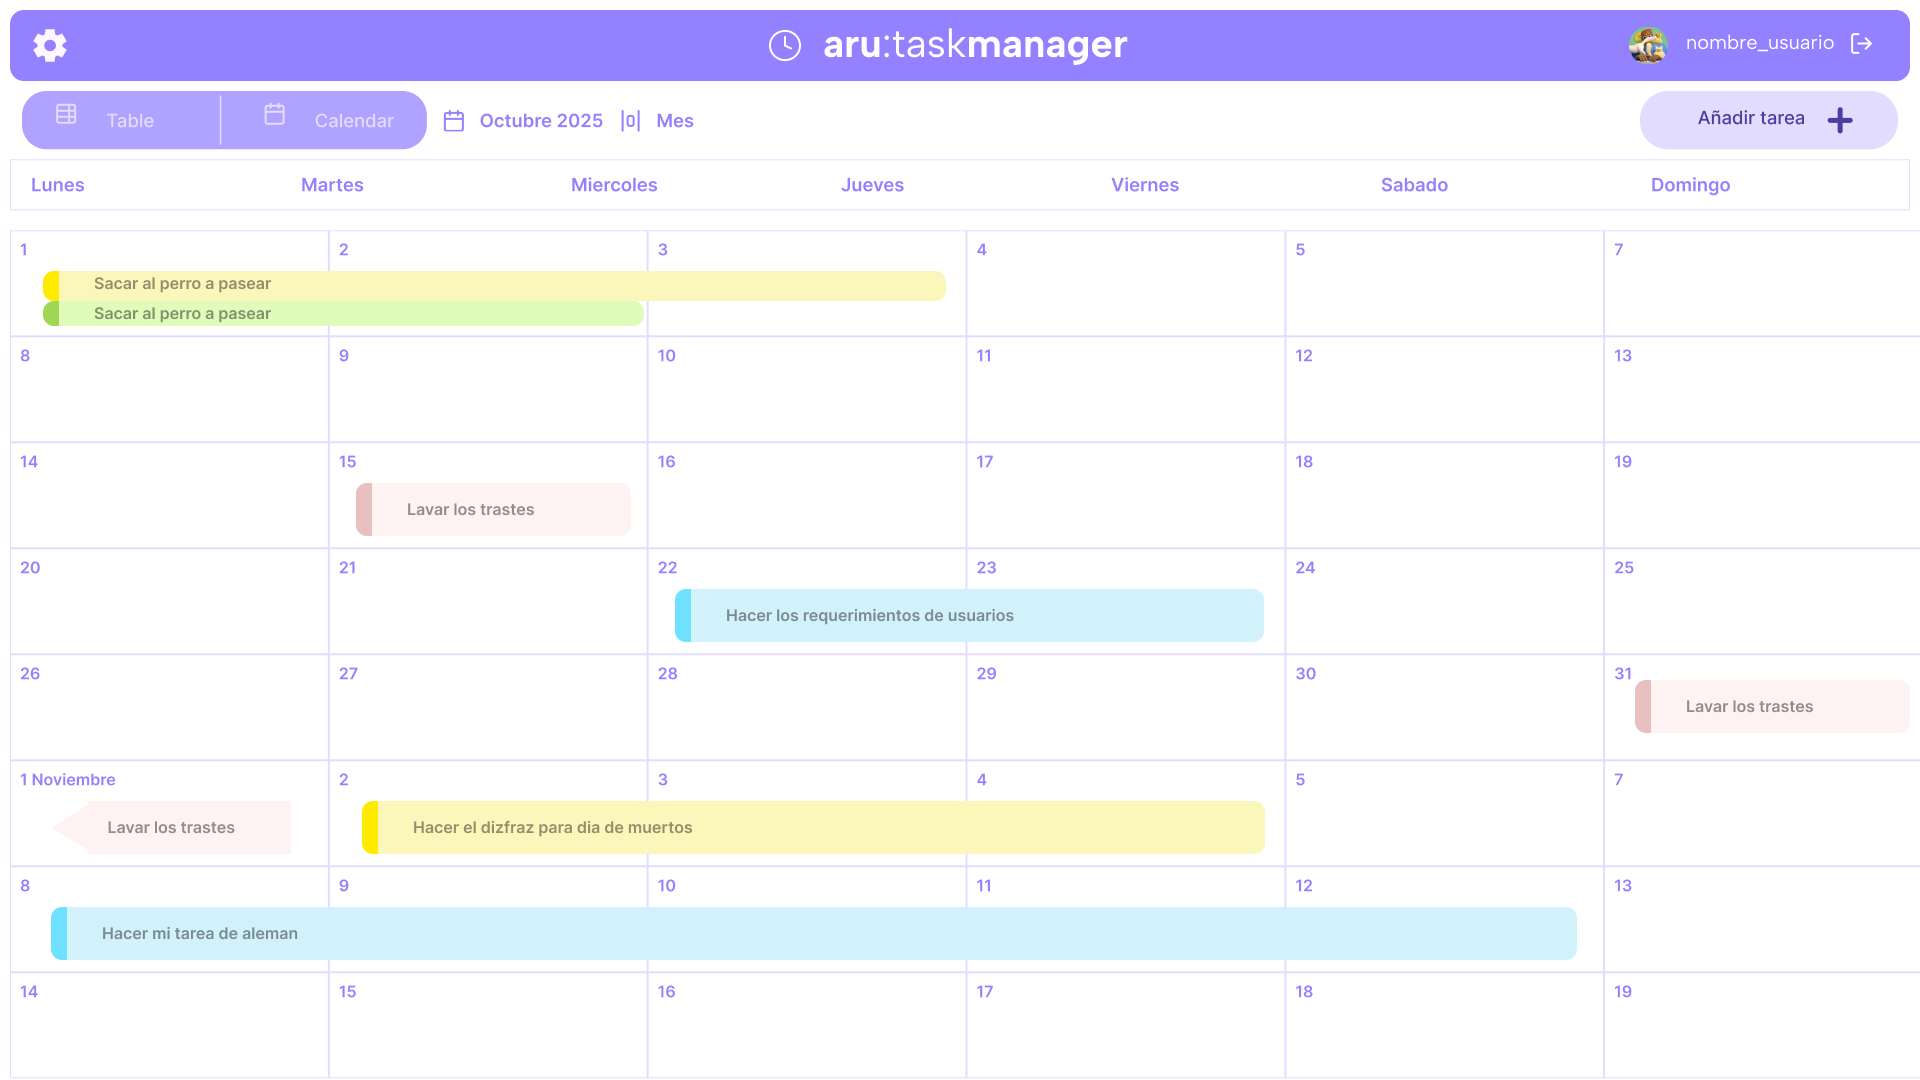
\includegraphics[width=0.85\linewidth]{pantallas/calendar.png}}
    \caption{Maqueta de la interfaz de usuario - Pantalla principal}
\end{figure}
\begin{figure}[H]
    \centering
    \fbox{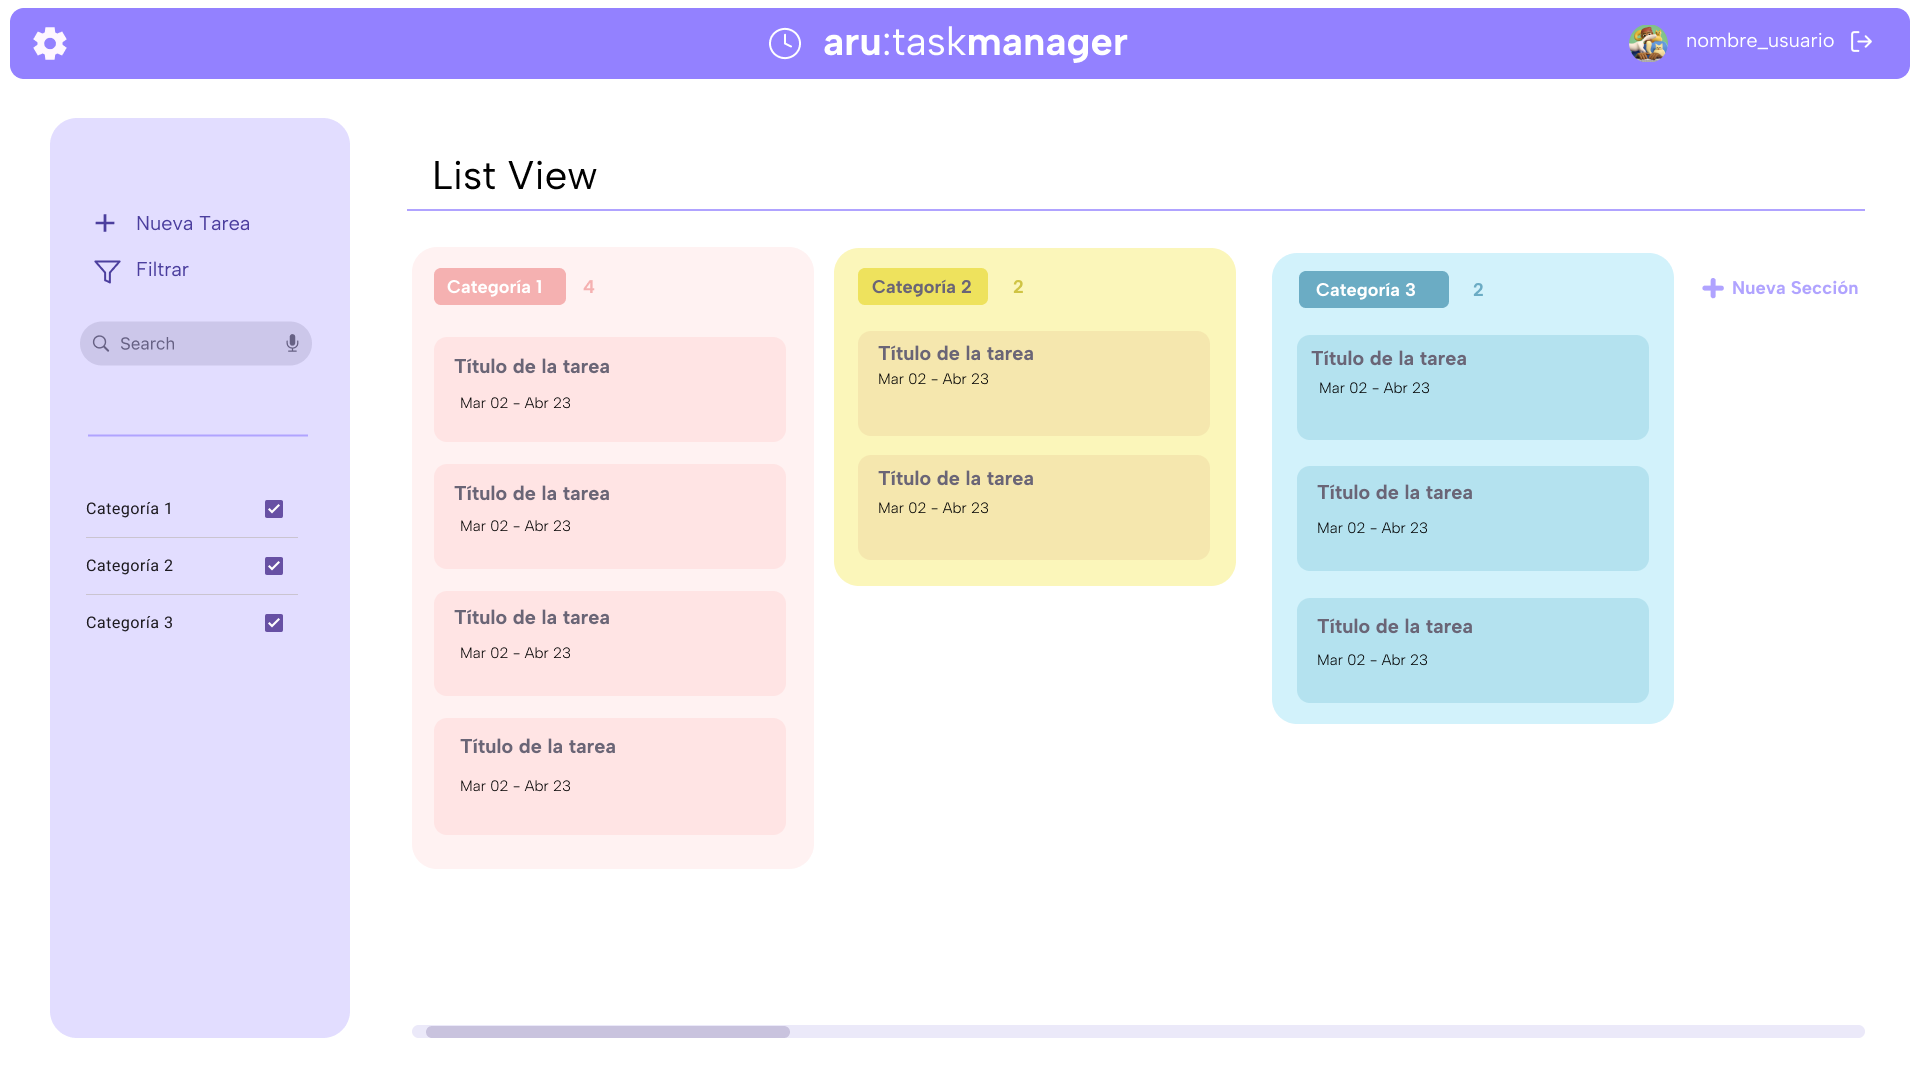
\includegraphics[width=0.85\linewidth]{pantallas/list_view.png}}
    \caption{Vista de Lista de Tareas}
\end{figure}
\begin{figure}[H]
    \centering
    \fbox{\includegraphics[width=0.6\linewidth]{pantallas/Modal para añadir tarea.png}}
    \caption{Modal para Agregar Nueva Tarea}
\end{figure}

\begin{figure}[H]
    \centering
    \fbox{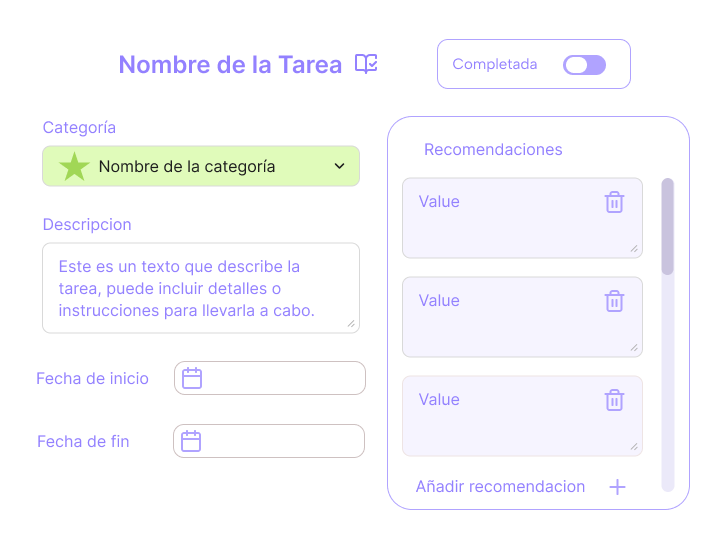
\includegraphics[width=0.6\linewidth]{pantallas/Modal para ver tarea.png}}
    \caption{Modal para Ver Detalles de Tarea y Recomendaciones}
\end{figure}
\begin{figure}[H]
    \centering
    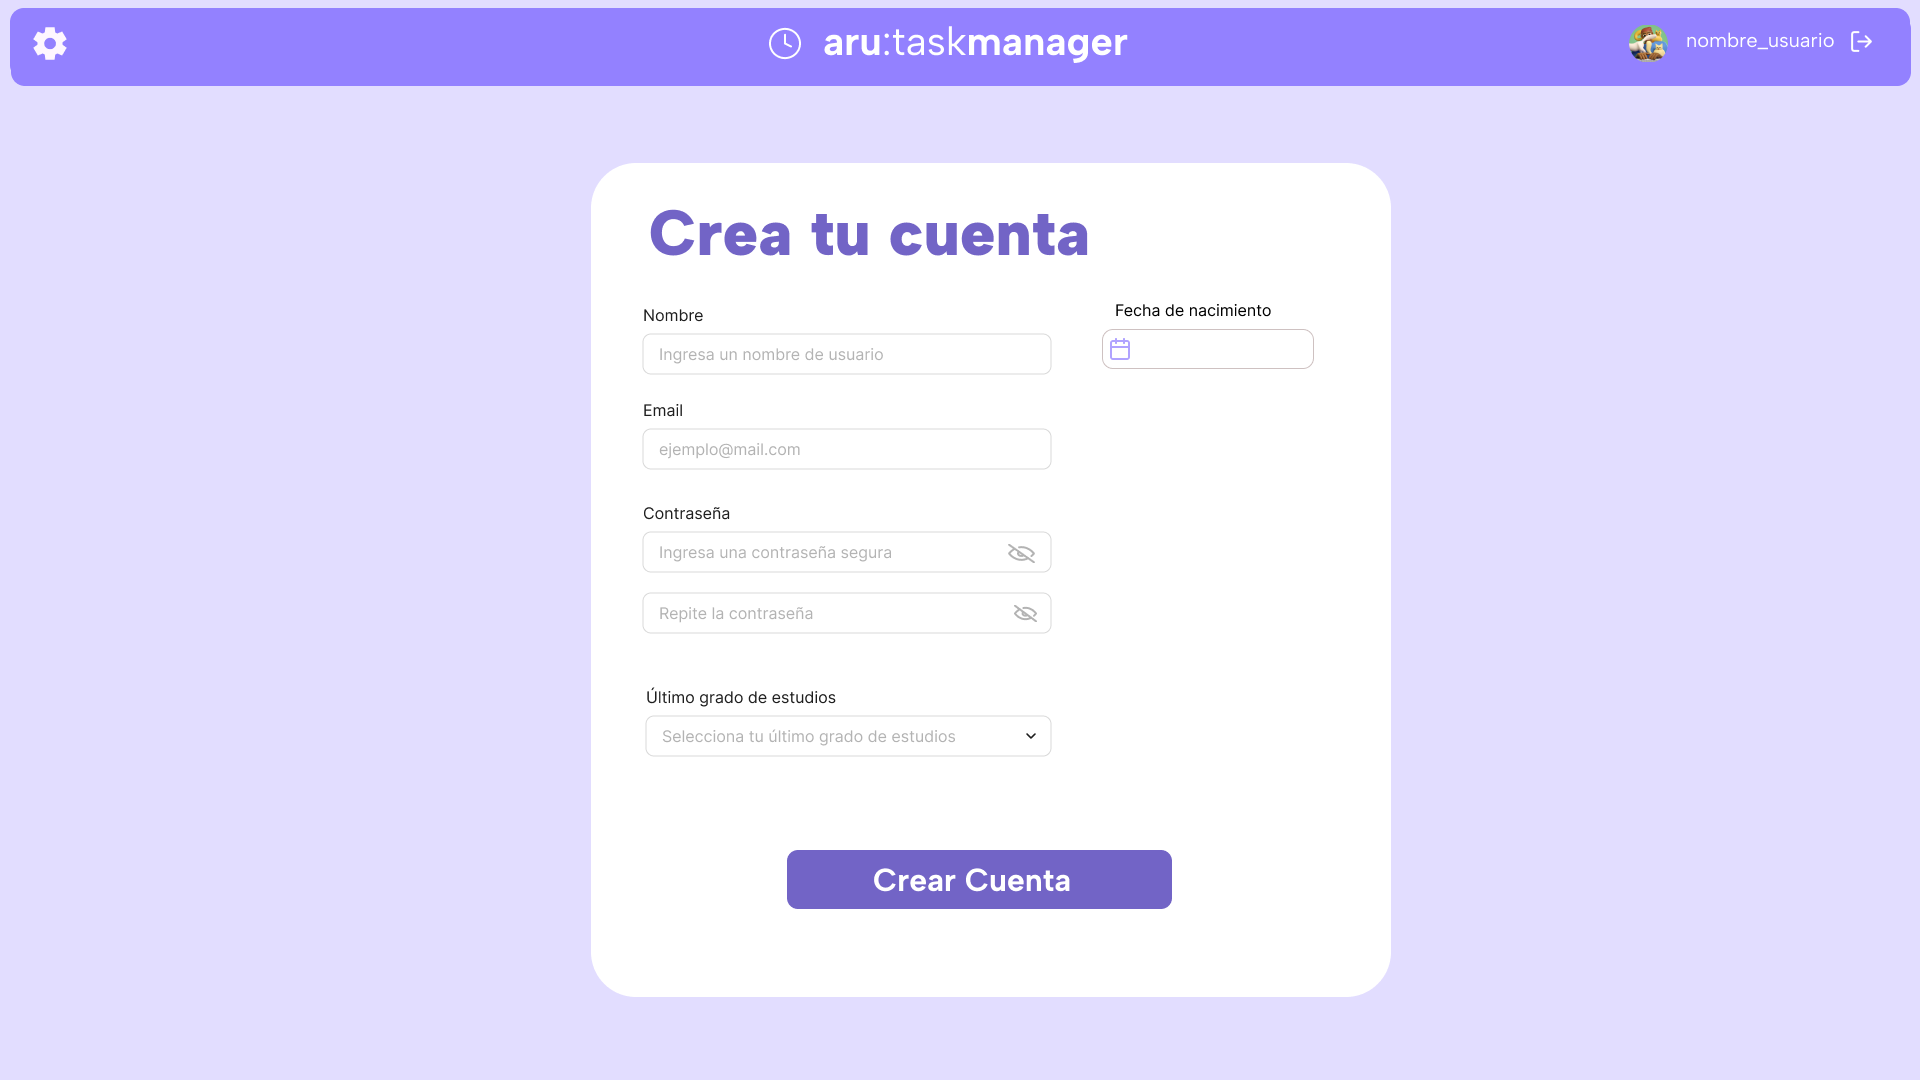
\includegraphics[width=\linewidth]{pantallas/register.png}
    \caption{Pantalla para crear una cuenta}
\end{figure}
\begin{figure}[H]
    \centering
    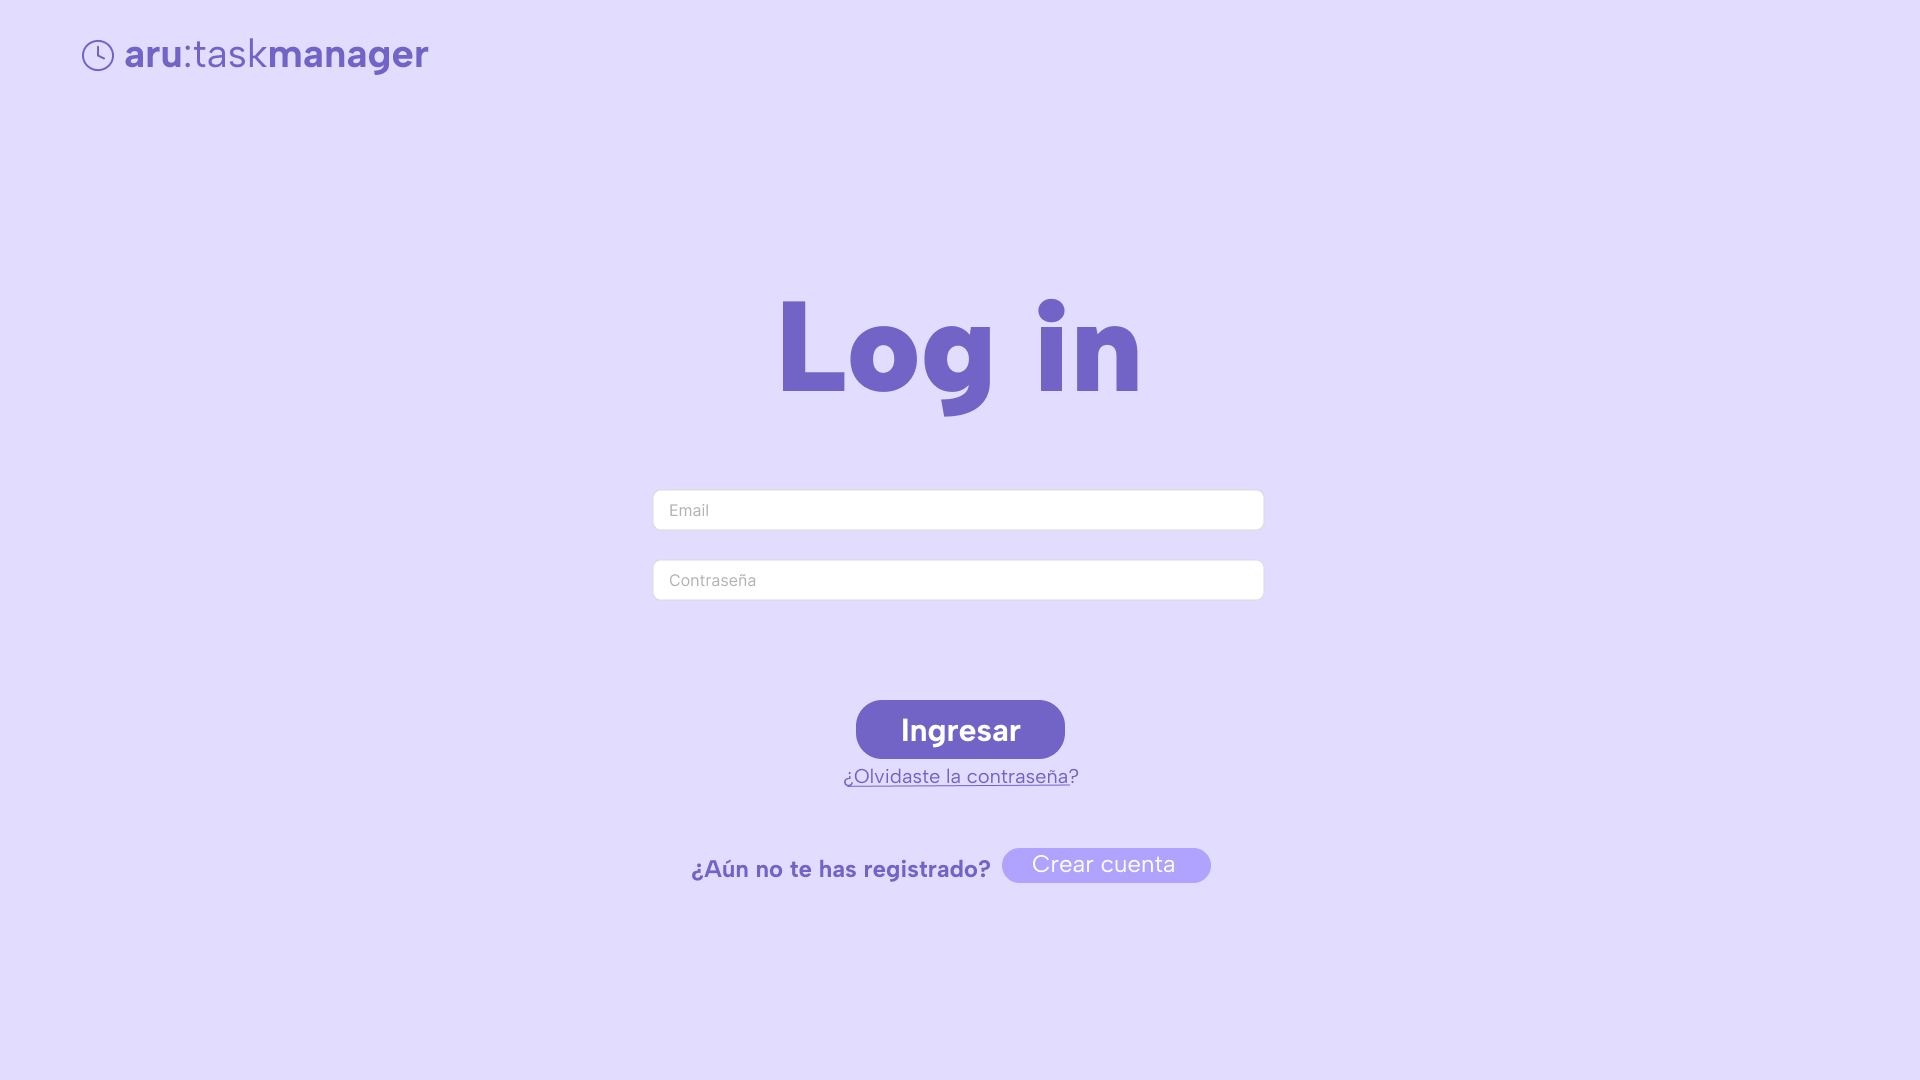
\includegraphics[width=\linewidth]{pantallas/login.png}
    \caption{Pantalla para iniciar sesión}
\end{figure}
\begin{figure}[H]
    \centering
    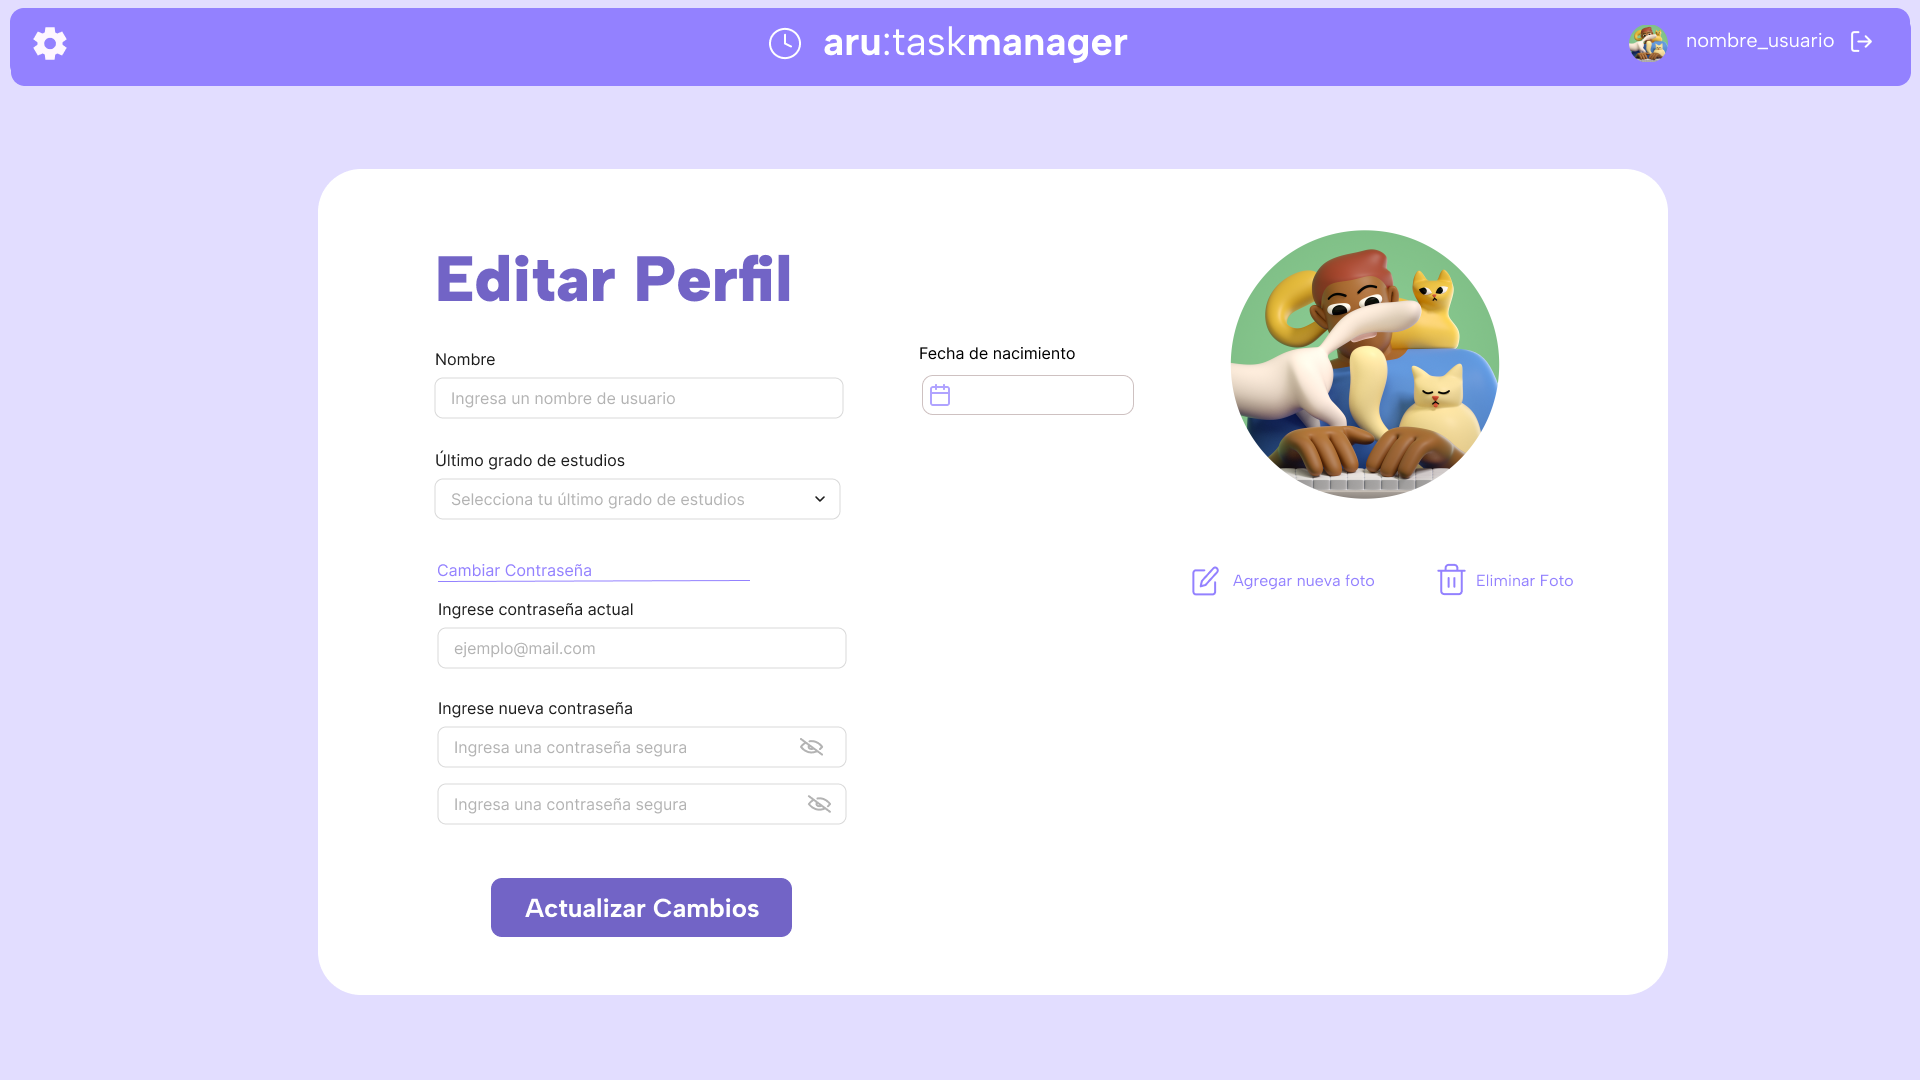
\includegraphics[width=\linewidth]{pantallas/Editar Perfil.png}
    \caption{Pantalla de Perfil de Usuario}
\end{figure}

\pagestyle{fancy}


%mmdc -i diagramas/nombre_archivo.mmd -o pngs/nombre_archivo.png -b transparent -t default

%%%%%%%%%% BIBLIOGRAFÍA %%%%%%%%%%%%%%%%%%%%%
\pagebreak
\printbibliography[heading=bibintoc]

\end{document}